\documentclass[10pt, letterpaper]{report}
% !TeX program = xelatex
%==================PREAMBOLO=======================%
\usepackage[utf8]{inputenc}
\usepackage{psvectorian}
\usepackage{pgfplots}
\usepackage[Rejne]{fncychap}
\usepackage[export]{adjustbox}
\usepackage[T1]{fontenc}
\usepackage{lmodern}
\usepackage{blindtext}
\usepackage{pdfpages}
\usepackage[shortlabels]{enumitem}
\usepackage{moresize}
\usepackage{graphicx} % Required for inserting images
\usepackage{hyperref}
\usepackage{listings}
\usepackage[table,xcdraw]{xcolor}
\usepackage{amssymb}
\usepackage{amsmath}
\usepackage[english]{babel}
\usepackage{nicefrac, xfrac}
\usepackage{tikz}
\usepackage{tikz-3dplot}
\usepackage{tikz-cd}
\usepackage{mathrsfs} 
\usepackage{titletoc}
\usepackage{fancyhdr}
\usepackage{psvectorian,lipsum}
\usepackage{fourier-orns}
\usepackage{lipsum}
\usepackage{wrapfig}
\usepackage{multicol}
\usepackage[paper=a4paper,left=25mm,right=25mm,bottom=25mm,top=25mm]{geometry}
\definecolor{light-gray}{gray}{0.95}
\definecolor{cop}{HTML}{f7ecd7}
\definecolor{copAut}{HTML}{ababab}
\definecolor{copAut2}{HTML}{c3c3e6}
\definecolor{purcop}{HTML}{d0d3db}
\definecolor{sapienza}{HTML}{660f1d}
\definecolor{lightSapienza}{HTML}{e3d3d5}
\definecolor{darkgreen}{HTML}{008000}
\definecolor{cartaRiciclata}{HTML}{fcfcf7}
\newcommand{\redText}[1]{\color{red}#1\color{black}}
\newcommand{\code}[1]{\colorbox{light-gray}{\texttt{#1}}}
\newcommand{\codee}[1]{\colorbox{white}{\texttt{#1}}}
\newcommand{\K}{{\mathbb K}}
\newcommand{\notimplies}{%
  \mathrel{{\ooalign{\hidewidth$\not\phantom{=}$\hidewidth\cr$\implies$}}}}
\newcommand{\flowerLine}{ \begin{center}\decofourleft\hphantom{ }\decoone\hphantom{ }\decofourright\hphantom{}\hphantom{aa}
\decofourleft\hphantom{ }\decoone\hphantom{ }\decofourright\hphantom{}\hphantom{aa}
\decofourleft\hphantom{ }\decoone\hphantom{ }\decofourright\hphantom{}\hphantom{aa}
\decofourleft\hphantom{ }\decoone\hphantom{ }\decofourright\hphantom{}\hphantom{aa} 
\decofourleft\hphantom{ }\decoone\hphantom{ }\decofourright\hphantom{}\hphantom{aa}
\decofourleft\hphantom{ }\decoone\hphantom{ }\decofourright\hphantom{}\hphantom{aa}
\decofourleft\hphantom{ }\decoone\hphantom{ }\decofourright\hphantom{}\hphantom{aa}
\decofourleft\hphantom{ }\decoone\hphantom{ }\decofourright\hphantom{}\hphantom{aa}
\decofourleft\hphantom{ }\decoone\hphantom{ }\decofourright\hphantom{}\hphantom{aa}
\end{center}}
\definecolor{g}{RGB}{60, 50, 50}
\newcommand{\textg}[1]{\color{g}{\textbf{#1}}\color{black}}
\newcommand{\teo}[1]{{\large\color{sapienza}\textbf{Teorema #1 :\hphantom{a}}}}
\newcommand{\defi}[1]{{\large\color{sapienza}\textbf{Definizione #1 :\hphantom{a}}}}
\newcommand{\claim}[1]{{\color{sapienza}\textbf{Claim #1 :\hphantom{a}}}}
\newcommand{\lemma}[1]{{\color{sapienza}\textbf{Lemma #1 :\hphantom{a}}}}
\newcommand{\dimo}[1]{{\color{sapienza}\textbf{Dimostrazione #1 :\hphantom{a}}}}
\newcommand{\prop}[1]{{\color{sapienza}\textbf{Proposizione #1 :\hphantom{a}}}}
\newcommand\greybox[1]{%
  \vskip\baselineskip%
  \par\noindent\colorbox{light-gray}{%
    \begin{minipage}{\textwidth}#1\end{minipage}%
  }%
  \vskip\baselineskip%
}
\newcommand\sapbox[1]{%
  \vskip\baselineskip%
  \par\noindent\colorbox{lightSapienza}{%
    \begin{minipage}{\textwidth}#1\end{minipage}%
  }%
  \vskip\baselineskip%
}
\newcommand{\ridFunc}{{f:\Sigma^*\rightarrow \Sigma^*}}
\newcommand{\rid}{{\le_m^P}}
\newcommand{\Z}{{\mathbb Z}}
\newcommand{\blank}{{\sqcup}}
\newcommand{\Prob}{{\mathbb P}}
\newcommand{\R}{{\mathbb R}}
\newcommand{\VA}{{\mathbb E}}
\newcommand{\N}{{\mathbb N}}
\newcommand{\quat}{{\mathbb H}}
\newcommand{\C}{{\mathbb C}}
\newcommand{\Sn}{{\mathcal S_n}}
\newcommand{\An}{{\mathcal A_n}}
\newcommand{\E}{{\mathcal E}}
\newcommand{\B}{{\mathcal B}}
\newcommand{\mcm}{{\text{mcm}}}
\newcommand{\rg}{{\text{rg}}}
\newcommand{\ve}{{\bar v}}
\newcommand{\spaz}{{\text{\hphantom{aa}}}}
\newcommand{\MCD}{{\text{MCD}}}
\newcommand{\tc}{{\text{ tale che }}}
\newcommand{\supp}{{\text{Supp}}}
\newcommand{\acc}{\\\hphantom{}\\}
\newcommand{\esempio}[1]{{\acc\large\color{sapienza}\textbf{Esempio #1 \hphantom{a}}\acc}}
\newcommand{\bra}[1]{\langle #1 \rangle}
\newcommand{\aut}{{\text{Aut}}}
\newcommand{\Span}{{\text{Span}}}
\newcommand{\End}{{\text{End}}}
\newcommand{\cen}{{\text{Centro}}}
\newcommand{\norm}{{\unlhd}}
\newcommand{\ciclS}{{\left \langle }}
\newcommand{\ciclE}{{\right \rangle }}
\newcommand{\boxedMath}[1]{\begin{tabular}{|c|}\hline \texttt{#1} \\ \hline\end{tabular} :} 
\newcommand{\shell}[1]{\colorbox{black}{\textcolor{white}{\texttt{#1}}}}
\newcommand{\eqImportante}[1]{\begin{center}\huge\lefthand\hphantom{a}
    \normalsize\texttt{#1}
    \hphantom{aaa}\huge\righthand\end{center}}

\fancyhf{}
\pagestyle{fancy}
\usepackage{pgf-pie}  
\usetikzlibrary{positioning}

\renewcommand{\headrule}{%
\vspace{-8pt}\hrulefill
\raisebox{-2.1pt}{\quad\decothreeleft\decotwo\decothreeright\quad}\hrulefill}

%sta roba serve per il codice C
\definecolor{mGreen}{rgb}{0,0.6,0}
\definecolor{mGray}{rgb}{0.5,0.5,0.5}
\definecolor{mPurple}{rgb}{0.58,0,0.82}
\definecolor{backgroundColour}{rgb}{0.95,0.95,0.92}

\lstdefinestyle{CStyle}{
    backgroundcolor=\color{backgroundColour},   
    commentstyle=\color{mGreen},
    keywordstyle=\color{magenta},
    numberstyle=\tiny\color{mGray},
    stringstyle=\color{mPurple},
    basicstyle=\footnotesize,
    breakatwhitespace=false,         
    breaklines=true,                 
    captionpos=b,                    
    keepspaces=true,                 
    numbers=left,                    
    numbersep=5pt,                  
    showspaces=false,                
    showstringspaces=false,
    showtabs=false,                  
    tabsize=2,
    language=C
}
\lstdefinestyle{CppStyle}{
    backgroundcolor=\color{backgroundColour},   
    commentstyle=\color{mGreen}\ttfamily,
    morecomment=[l][\color{magenta}]{\#}
    keywordstyle=\color{blue}\ttfamily,
    numberstyle=\tiny\color{mGray},
    stringstyle=\color{red}\ttfamily,
    basicstyle=\ttfamily,
    breakatwhitespace=false,         
    breaklines=true,                 
    captionpos=b,                    
    keepspaces=true,                 
    numbers=left,                    
    numbersep=5pt,                  
    showspaces=false,                
    showstringspaces=false,
    showtabs=false,                  
    tabsize=2,
    language=C
}
\lstset{language=C++,
                basicstyle=\ttfamily,
                keywordstyle=\color{blue}\ttfamily,
                stringstyle=\color{red}\ttfamily,
                commentstyle=\color{green}\ttfamily,
                morecomment=[l][\color{magenta}]{\#}
}
%fine roba che serve per il codice C
\usepackage{minted}
\usepackage{algorithm}
\usepackage{algpseudocode}
\newcommand{\titolo}{Machine Learning }

 %TOGLI COMMENTO SE USI XELATEX
%\usepackage{fontspec}
\title{\titolo} %========TITOLO========%
\author{Marco Casu}
\date{\vspace{-5ex}}
\begin{document}

%==================COPERTINA=======================%
\begin{titlepage}
    
\begin{center}
    %TOGLI COMMENTO SE USI XELATEX
   %\setmainfont{Palace Script MT}
   \HUGE Marco Casu\acc
\end{center}
\thispagestyle{empty}
\begin{figure}[h]
    \centering{
        %l'immagine deve avere una risoluzione 2048x2048
        
\includegraphics[width=1\textwidth ]{images/Copertina.png}
    }
\end{figure}
\vfill 
\centering 
\includegraphics[width=0.4\textwidth ]{../../preamble/Stemma_sapienza.png} \acc
\centering \Large \color{sapienza}Faculty of Information Engineering, Computer Science and Statistics\\
Department of Computer, Control and Management Engineering\\
Master's degree in Artificial Intelligence and Robotics
\end{titlepage}

%===================FINE COPERTINA======================%
\newpage
%\pagecolor{cartaRiciclata}%\setmainfont{Algerian}
\Large
This document summarizes and presents the topics for the \titolo course for the Master's degree in Artificial Intelligence and Robotics at Sapienza University of Rome. The document is free for any use. If the reader notices any typos, they are kindly requested to report them to the author.
\vfill
\begin{figure}[h!]
    \raggedright
    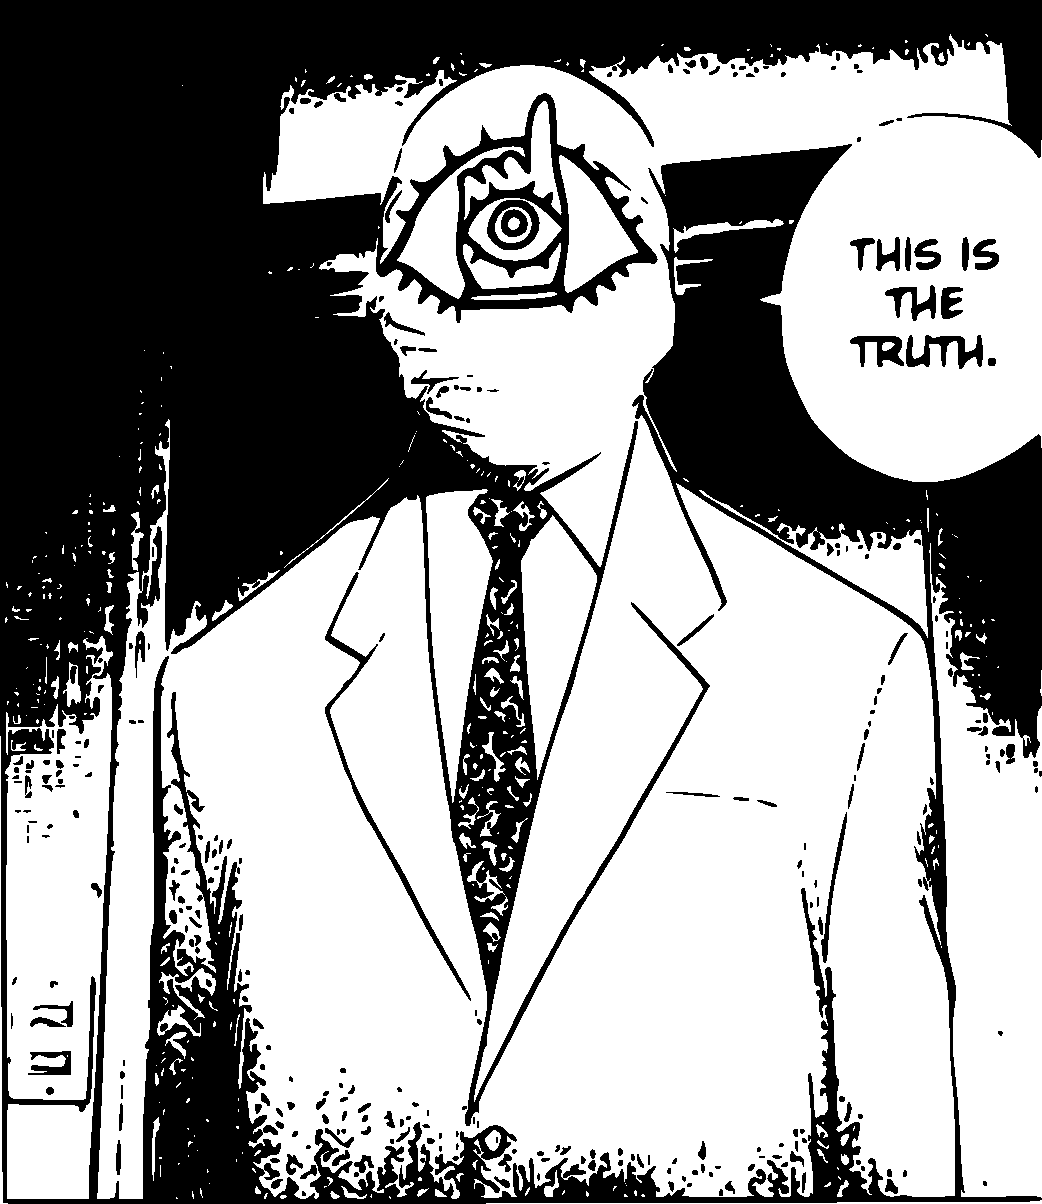
\includegraphics[width=0.4\textwidth,right ]{../../preamble/tomodachi.pdf} 
\end{figure}
\newpage %\setmainfont{Times New Roman}
\normalsize

\tableofcontents 
\newpage

%==================FOOTER e HEADER=======================%
\fancyhf{}
\fancyhead[L]{\nouppercase{\leftmark}}
\fancyhead[R]{Sezione \thesection}
\fancyfoot[C]{\thepage}
\fancyfoot[L]{\titolo}
\fancyfoot[R]{ Marco Casu}
%\fancyfoot[R]{\setmainfont{Palace Script MT}\huge Marco Casu \setmainfont{Times New Roman}}
%==================FOOTER e HEADER=======================%

\newtheorem{definition}{Definition}

%==================INIZIO======================%
\chapter{Introduction}
\section{Basic Definition of a ML Problem}
In this chapter we will introduce the basics of what is a machine learning problem, giving a mathematical definition. informally, with machine learning we define the use of knowledge (data) to improve the performance of a given program, using past experiences.\bigskip

Generally, we use machine learning to solve problems with no deterministic solutions, trying to find an approximate one (such as recognizing what animal is represented in a given photo).\bigskip 

Usually, a machine learning problem consists in three main component:\begin{itemize}
    \item $T$ : the given task
    \item $P$ : a performance metric
    \item $E$ : the past experiences (the data)
\end{itemize}
Let's see an example, we want to model a program capable of playing \textit{Checkers}.
\begin{center}
    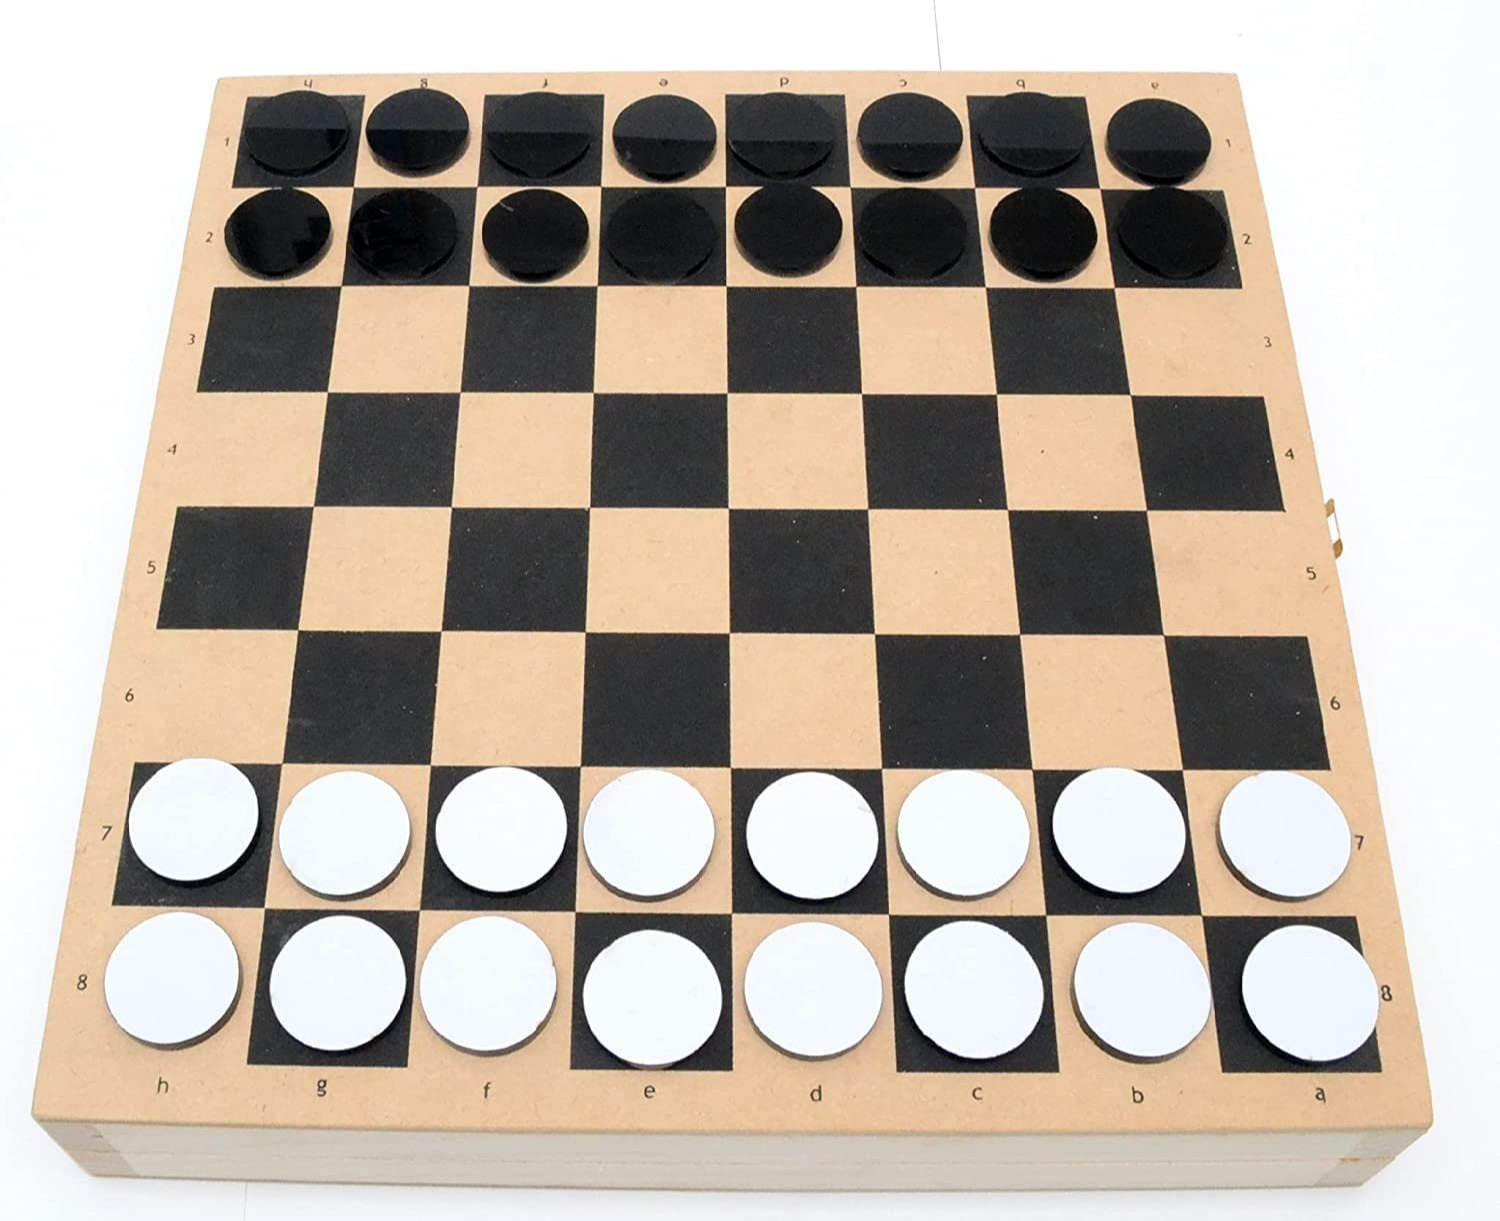
\includegraphics[width=0.35\textwidth]{images/Checkers.jpg}
\end{center}
The task $T$ is to play the game, the performance metric $P$ measure the ratio of win in a tournament, and the experiences is given by the past match. We can create this matches by letting the computer play against himself, or by making it play against a human. We can consider two types of target functions that models the behavior of the model:\begin{itemize}
    \item $ChooseMove : Board\rightarrow Move$
    \item $V : Board\rightarrow\R$
\end{itemize}
$Board$ is the set of the possible board configurations, move is the set of feasible moves. The image of the function $V$ should represents the validity of a board in the following sense:\begin{itemize}
    \item if $b\in Boards$ is a configuration that represents the win of the player, then $V(b)=1$
    \item else if $b\in Boards$ is a configuration that represents the win of the opponent, then $V(b)=-1$
    \item else if $b\in Boards$ is a configuration that represents a draw, then $V(b)=0$
    \item else, $V(b)=V(b')$ where $b'$ is
the best final board state that can be achieved starting from $b$ and
playing optimally until the end of the game.
\end{itemize}
The function $V$ can be used to predict the next move by considering all possible boards that can be obtained from the feasible moves.
We focus on the function $V$, this should be an optimal model, but is not computable, because we cannot tell if a play is ''optimal'' (this is the goal of the model), so we want to consider a function that approximate the behavior of $V$.\bigskip

We consider a function $\hat V: Board\rightarrow\R$ defined as follows:\begin{equation}
    \hat V(b)=\sum_{i=0}^6w_if_i(b)
\end{equation}
where $\mathbf w = (w_i)$ is real coefficients, and the functions $f_i$ represents some features of the given board:\begin{itemize}
    \item $f_1(b)$ : number of black pieces on $b$
    \item $f_2(b)$ : number of red pieces on $b$
    \item ecc...
\end{itemize}
We don't know if some features are useful to predict which move is optimal, is important that this features model the knowledge of the \textit{domain} (in this case, the game of Checkers). \bigskip

with \textit{learning the function} $\hat V$, we intend to finds the coefficients $\mathbf w$ which make the function $\hat V$ more similar to $V$ as possible. There are various method to find these coefficients.\bigskip

Let's introduce some notation:\begin{itemize}
    \item with $V$ we  define the \textbf{target function} (always unknown and uncomputable).
    \item with $\hat V$ we  define the \textbf{learned function}, the approximation of $V$ that we want to find.
    \item with $V_{train}(b)$ we define the value of $V$ obtained at $b$, where $b$ is a part of a data set that is given. We will use the values of $V_{train}$ on the data set to synthesize $\hat V$.
    \item with $D$ we define the given data set:\begin{equation}
        D=\bigcup_{i=1}^n\{b_i,V_{train}(b_i)\}
    \end{equation}
    $n$ is the number of the available data.
\end{itemize}
The iterative method given in the Algorithm \ref{alg:LMS} is an informal example of how we can find the values for $\mathbf w$.
\begin{algorithm}
    \caption{LMS weight update rule}\label{alg:LMS}
    \begin{algorithmic}
    \Require $D$, $V_{train}$, $k$
    \State initialize $\mathbf w$ with small random values 
    \For{$k$ times}  
    \State select a sample $b$ from $D$
    \State $error(b)=V_{train}(b)-\hat V(b)$
    \For{each feature $i$} 
    \State $w_i\leftarrow w_i+c\cdot f_i(b)\cdot error(b)$
    \EndFor
    \EndFor
    \end{algorithmic}
\end{algorithm}
In this case $c$ is a small constant, usually in $(0,1]$, to moderate the rate of learning.\bigskip

The function $error(b)$ is computable only on the sample $b$ given in the dataset $B$, the goal of the method is to converge to a local minimum for the function  \begin{equation}
    \sum_{b_i\in D}error(b_i).
\end{equation}
Once we synthesize $\hat V$ with this method, we can make the model play against human and track the result to use it as an additional dataset. The diagram in image \ref{img:DesignChoice} represents the process of designing an artificial intelligence agent.

\begin{figure}[h!]
    \centering
    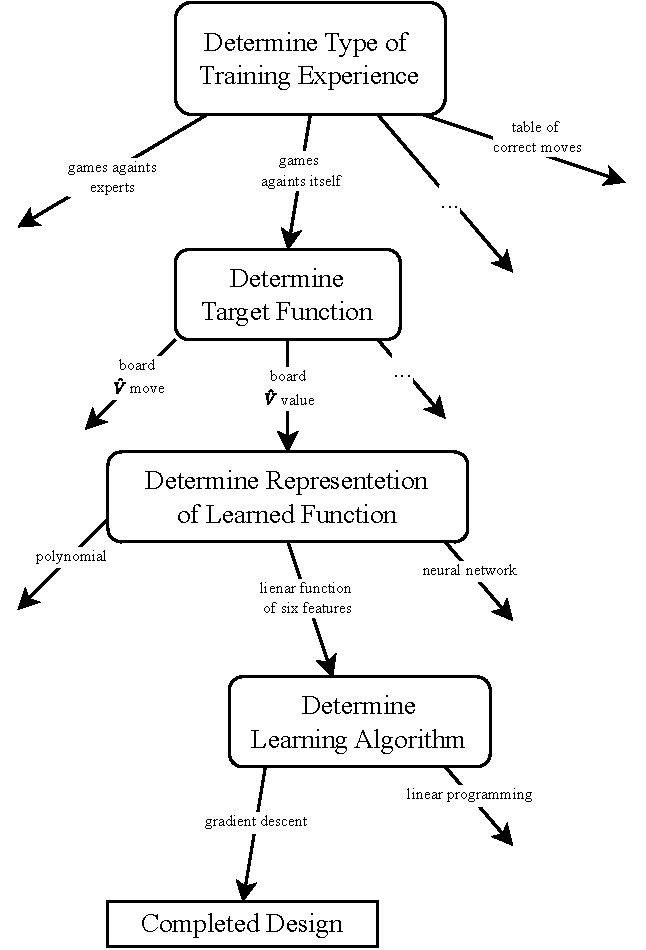
\includegraphics[width=0.35\textwidth]{images/DesignChoice.pdf}
    \caption{Design Choices}
    \label{img:DesignChoice}
\end{figure}
\section{Types of Machine Learning Problems}
There are different types of machine learning problems:\begin{itemize}
    \item Supervised Learning\begin{itemize}
        \item Classification
        \item Regression
    \end{itemize}
    \item Unsupervised Learning
    \item Reinforcement Learning
\end{itemize}

\begin{definition}
    Given a function $f:X\rightarrow Y$, and a training set $X_D\subset X$ containing information about $f$, \textbf{learning} the function $f$ means computing an approximated function $\hat f$ such that is much close as possible to $f$ on $X$\begin{equation}
        \hat f(x)\simeq f(x), \ \ x\in X
    \end{equation}
    more formally, we want to find $\hat f$ that minimize the following integral:\begin{equation}
        \int_{X}|\hat f(x)-f(x)|dx
    \end{equation}
    if $X\subseteq \R^n$ and is uncountable, and 
    \begin{equation}
        \sum_{x\in X}|\hat f(x)-f(x)|
    \end{equation}
    if $X$ is countable.
\end{definition}
This is not a simple problem, $f$ is not computable, so the difference $f-\hat f$, and $X$ is usually uncountable ora big set, way bigger than the training set $X_D$. \bigskip

Machine learning problems can be classified in terms of the input data set $D$, given a target function $f:X\rightarrow Y$ a problem is\begin{itemize}
    \item a \textbf{supervised learning} problem if $D=\bigcup_{i=1}^n\{(x_i,y_i)\}\subset X\times Y$ .
    \item an \textbf{unsupervised learning} problem if $D=\bigcup_{i=1}^n\{(x_i)\}\subset X$.
    \item a \textbf{reinforcement learning} problem, the condition on the input dataset will be discussed later.
\end{itemize}
The problems can also be classified in terms of the target function $f:X\rightarrow Y$
\begin{align*}
   & X=\begin{cases}
        A_1\times \dots \times A_m, \ A_i \text{ finite set} \ \ \textbf{(Finite Discrete Problem)}\\ 
        \R^n \ \ \textbf{(Continuous)}
    \end{cases}\\ 
    & Y=\begin{cases}
         \R^k \ \ \textbf{(Regression)}\\ 
        \{C_1,C_2\times C_k\} \ \ \textbf{(Classification)}
    \end{cases}
\end{align*}
special case (\textbf{Concept Learning}):\begin{align*}
    & X = A_1\times \dots \times A_m, \ A_i \text{ finite set}\\ 
    & Y = \{0,1\}
\end{align*}
Classification problems is also known as \textit{Pattern Recognition Problems}, the goal is to return the class to which a specific instance belong.\begin{center}
     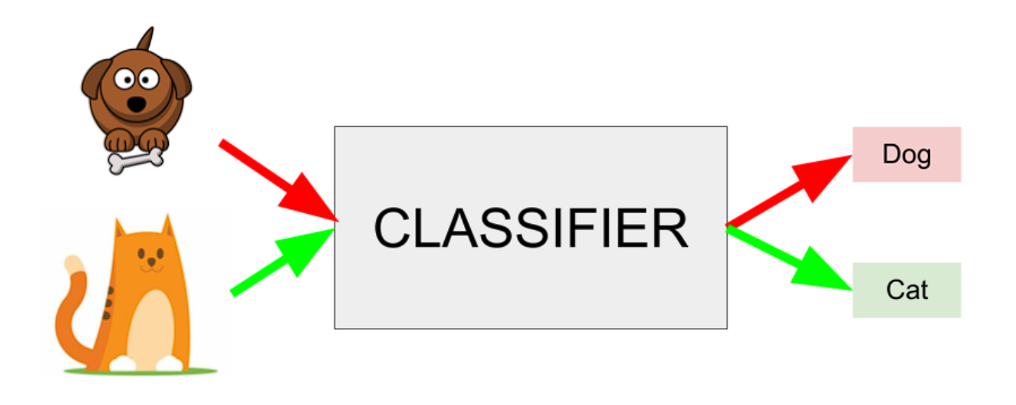
\includegraphics[width=0.6\textwidth]{images/classifier.png}
\end{center}
Some examples are:\begin{itemize}
    \item face/object/character recognition
    \item speech/sound recognition
    \item medical diagnosis
    \item document classification.
\end{itemize}
Regression problems consists in approximating real valued functions.
\begin{center}
     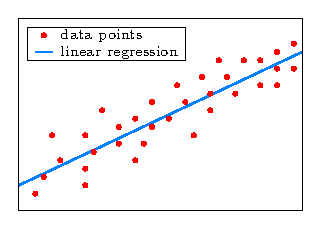
\includegraphics[width=0.35\textwidth]{images/regression.eps}
\end{center}
Unsupervised learning discovers data patterns without a specific output. The main goal is to understand what's normal in a dataset. \textit{Clustering} is a key technique that groups similar data points. Applications include customer segmentation, image compression, and bioinformatics motif learning.\bigskip

Reinforcement learning consists in
\end{document}